% LTeX: language=it

\documentclass{../.common/high-school-notebook}

\usetikzlibrary{calc,patterns,angles,quotes}

\hypersetup{
  pdftitle={Quaderno delle regole - Matematica},
  pdfauthor={Tommaso Bocchietti},
  pdfsubject={High School Notebook},
}


\begin{document}
\graphicspath{{../.common/}}

\title{Quaderno delle regole - Matematica}
\author{Tommaso Bocchietti}

\maketitle

\begin{figure}[H]
  \centering
  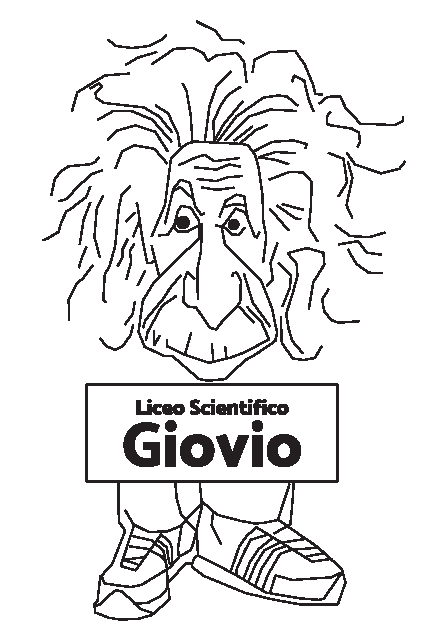
\includegraphics[width=0.7\textwidth]{../.common/Einstein_Logo}
  \label{fig:Einstein_Logo}
\end{figure}


\pagebreak
\tableofcontents

% \pagebreak
% % LTeX: language=it

\section{Piano cartesiano}

% \pagebreak
% % LTeX: language=it

\section{Equazioni e disequazioni con moduli e radici irrazionali}
% % LTeX: language=it

\section{Funzioni}
% % LTeX: language=it

\section{Successioni numeriche}
% % LTeX: language=it

\section{Piano cartesiano (coniche)}

\pagebreak
% LTeX: language=it

\section{Goniometria}

Un angolo può essere misurato in gradi o radianti, infatti si ha $\alpha^{\circ}=\alpha[rad] \frac{180^{\circ}}{\pi}$.
Considerando una circonferenza goniometrica (raggio $r=1$), un angolo orientato $\alpha$, dal prolungamento del lato dell'angolo $\alpha$, otteniamo l'intersezione $B$, dove:

\begin{figure}[h]
    \centering
    % \begin{tikzpicture}
    %     \begin{axis}[
    %             unit vector ratio* = 1 1 1,
    %             clip=false,
    %             width=\textwidth,
    %             height=0.5*\textwidth,
    %             axis lines = middle,
    %             ymax=1.5,
    %             ymin=-1.5,
    %             xmax = 1.5,
    %             xmin = -1.5,
    %             xtick = {-1, 0, 1},
    %             ytick = {-1, 0, 1}
    %         ]
    %     \end{axis}
    %     % \draw (-1,0) node[left] {$(-1,0)$} -- (1,0) node[right] {$(1,0)$};
    %     % \draw (0,-1) node[below] {$(0,-1)$} -- (0,1) node[above] {$(0,1)$};
    %     \draw (center) coordinate (O) circle (1);
    %     \draw[red, very thick] (30:1cm) coordinate (B) -- (0,0-|B) coordinate(Bx) node[midway,left]{$\sin\alpha$};
    %     \draw [very thick,orange] (1,0) -- (intersection cs: first line={(O)--(B)},second line={(3,0)--(3,3)}) coordinate(B') node[midway,right]{$\tan\alpha$};
    %     \draw (O) -- (B');
    %     \draw[very thick,blue] (O) -- (Bx) node[midway,below]{$\cos\alpha$};
    % \end{tikzpicture}
    \begin{tikzpicture}[scale=2]
        \draw[step=.5cm,gray,very thin] (-1.4,-1.4) grid (1.4,1.4);
        \filldraw[fill=blue!20,draw=red] (0,0) -- (3mm,0mm)
        arc [start angle=0, end angle=30, radius=3mm] -- cycle;
        \node[red] at (15:2mm) {$\alpha$};
        \draw[->] (-1.5,0) -- (1.5,0) coordinate (x axis)node[right]{$x$};
        \draw[->] (0,-1.5) -- (0,1.5) coordinate (y axis)node[above]{$y$};
        \draw (0,0) circle [radius=1cm];
        \draw[very thick,orange]
        (30:1cm) -- node[left=1pt,fill=white] {$\sin \alpha$} (30:1cm |- x axis);
        \draw[very thick,blue]
        (30:1cm |- x axis) -- node[below=2pt,fill=white] {$\cos \alpha$} (0,0);
        \path [name path=upward line] (1,0) -- (1,1);
        \path [name path=sloped line] (0,0) -- (30:1.5cm);
        \draw [name intersections={of=upward line and sloped line, by=t}]
        [very thick,red] (1,0) -- node [right=1pt,fill=white]
        {$\displaystyle \tan \alpha$} (t);
        \draw (0,0) -- (t);
        \foreach \x/\xtext in {-1, -0.5/-\frac{1}{2}, 1}
        \draw (\x cm,1pt) -- (\x cm,-1pt) node[anchor=north,fill=white] {$\xtext$};
        \foreach \y/\ytext in {-1, -0.5/-\frac{1}{2}, 0.5/\frac{1}{2}, 1}
        \draw (1pt,\y cm) -- (-1pt,\y cm) node[anchor=east,fill=white] {$\ytext$};
    \end{tikzpicture}
\end{figure}

$y_B = \sin(\alpha) \qquad x_B = \cos(\alpha)$
$\frac{y_B}{x_B} = \tan(\alpha)$

Al variare dell'angolo $\alpha$, le funzioni vengono così rappresentate:

\begin{figure}[h]
    \centering
    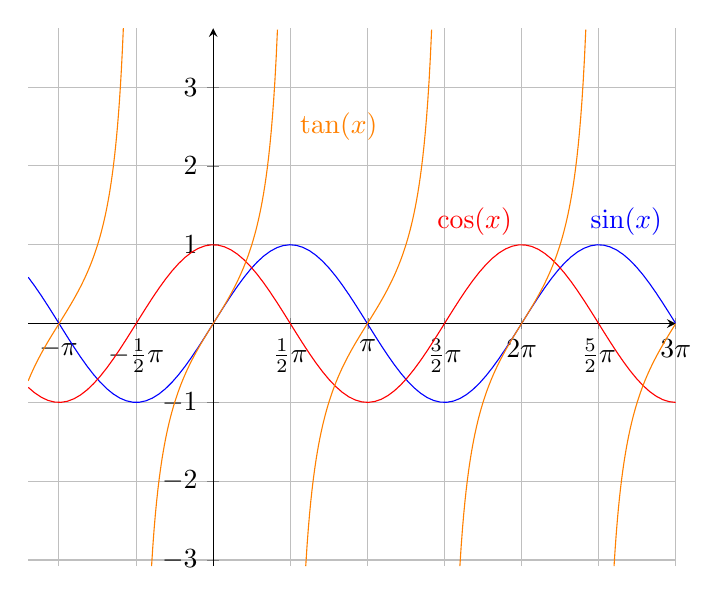
\begin{tikzpicture}
        \begin{axis}[enlargelimits=false,
                axis lines=middle,
                scale=1.2,
                xtick={-3.15159, -1.57080, 0,
                        1.57080,  3.15159, 4.71239,
                        6.28318,  7.85398, 9.42478 },
                xticklabels={$-\pi$, $-\frac{1}{2}\pi$, 0,
                        $\frac{1}{2}\pi$, $\pi$, $\frac{3}{2}\pi$,
                        $2\pi$, $\frac{5}{2}\pi$, $3\pi$ },
                ytick={-3,-2,-1,0,1,2,3},
                grid=major, % only a grid on the defined ticks
                samples=100 % number of points
            ]

            % sin
            \addplot[blue,no marks,domain=-1.2*pi:3*pi]{sin(deg(x))}; % deg to convert radians
            \node[right=10pt,above] at (axis cs:5*pi/2,1){\color{blue}$\sin(x)$};

            % cos
            \addplot[red,no marks,domain=-1.2*pi:3*pi] {cos(deg(x))};
            \node[above left] at (axis cs:2*pi,1){\color{red}$\cos(x)$};

            % tan, multiple parts because of singularities
            \addplot[orange,no marks,domain=-1.2*pi:-0.583*pi, ]{tan(deg(x))};
            \addplot[orange,no marks,domain=-0.4*pi:5*pi/12,   ]{tan(deg(x))};
            \addplot[orange,no marks,domain=27*pi/45:17*pi/12, ]{tan(deg(x))};
            \addplot[orange,no marks,domain=1.6*pi:29*pi/12,   ]{tan(deg(x))};
            \addplot[orange,no marks,domain=2.6*pi:36*pi/12,   ]{tan(deg(x))};
            \node[right] at (axis cs:pi/2,2.5){\color{orange}$\tan(x)$};

        \end{axis}
    \end{tikzpicture}
\end{figure}

Tutte queste funzioni sono periodiche, per cui $f(x) = f(x+T)$, dove $T$ è il periodo della funzione.

Angoli noti:

\begin{table}[h]
    \centering
    \begin{tabular}{|l|l|l|l|}
        \hline
        Angolo $^{\circ}$ & $\sin(\alpha)$        & $\cos(\alpha)$        & $\tan(\alpha)$       \\ \hline
        0                 & 0                     & 1                     & 0                    \\ \hline
        30                & $\frac{1}{2}$         & $\frac{\sqrt{3}}{2}$  & $\frac{1}{\sqrt{3}}$ \\ \hline
        45                & $\frac{\sqrt{2}}{2} $ & $\frac{\sqrt{2}}{2} $ & $1$                  \\ \hline
        60                & $\frac{\sqrt{3}}{2}$  & $\frac{1}{2}$         & $\sqrt{3}$           \\ \hline
        90                & 1                     & 0                     & $\infty$             \\ \hline
    \end{tabular}
\end{table}

Esistono poi le funzioni inverse, che permettono di trovare l'angolo $\alpha$ a partire da un dato valore della funzione (es. $\sin(30^{\circ}) = \frac{1}{2} \rightarrow 30^{\circ} = \arcsin(\frac{1}{2})$).

\begin{figure}[h]
    \centering
    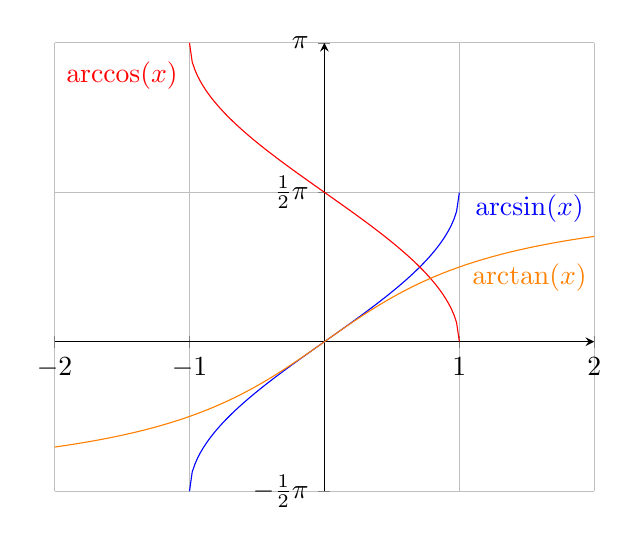
\begin{tikzpicture}
        \begin{axis}[enlargelimits=false,
                axis lines=middle,
                xtick={-2,-1,0,1,2},
                ytick={-1.570780, 1.570780, 3.14159},
                yticklabels={$-\frac{1}{2}\pi$,$\frac{1}{2}\pi$,$\pi$},
                grid=major,
                samples=100
            ]

            % arcsin
            \addplot[domain=-1:1,no marks,blue] {rad(asin(x))};
            \node at (axis cs:1.52,1.4){\color{blue}$\arcsin(x)$};

            % arccos
            \addplot[domain=-1:1,no marks,red] {rad(acos(x))};
            \node at (axis cs:-1.5,2.8){\color{red}$\arccos(x)$};

            % arctan
            \addplot[domain=-2:2,no marks,orange] {rad(atan(x))};
            \node at (axis cs:1.52,.67){\color{orange}$\arctan(x)$};

        \end{axis}
    \end{tikzpicture}
\end{figure}

Il periodo $T$ di una funzione si ricava come: $f(x)=\sin(\omega x) \rightarrow T=\frac{2\pi}{\omega}$

Relazioni fondamentali della goniometria: $\sin(\alpha)^2 + \cos(\alpha)^2 = 0$ e $\frac{\sin(\alpha)}{\cos(\alpha)} = \tan(\\alpha)$

\subsection{Funzioni goniometriche}

\subsubsection*{Addizione}

\begin{itemize}
    \item $\sin(\alpha+\beta)=\sin(\alpha)\cos(\beta)+\cos(\alpha)\sin(\beta)$
    \item $\cos(\alpha+\beta)=\cos(\alpha)\cos(\beta)-\sin(\alpha)\sin(\beta)$
    \item $\tan(\alpha+\beta)=\frac{\tan(\alpha)+\tan(\beta)}{1-\tan(\alpha)\tan(\beta)}$
\end{itemize}

\subsubsection*{Sottrazione}

\begin{itemize}
    \item $\sin(\alpha-\beta)=\sin(\alpha)\cos(\beta)-\cos(\alpha)\sin(\beta)$
    \item $\cos(\alpha-\beta)=\cos(\alpha)\cos(\beta)+\sin(\alpha)\sin(\beta)$
    \item $\tan(\alpha-\beta)=\frac{\tan(\alpha)-\tan(\beta)}{1+\tan(\alpha)\tan(\beta)}$
\end{itemize}

\subsubsection*{Duplicazione}

\begin{itemize}
    \item $\sin(2\alpha)=2\sin(\alpha)\cos(\alpha)$
    \item $\cos(2\alpha)=\cos^2(\alpha)-\sin^2(\alpha)$
    \item $\tan(2\alpha)=2\tan(\alpha)\frac{1-\tan^2(\alpha)}{1+\tan^2(\alpha)}$
\end{itemize}

\subsubsection*{Bisezione}

\begin{itemize}
    \item $\sin(\frac{\alpha}{2})=\sqrt{\frac{1-\cos(\alpha)}{2}}$
    \item $\cos(\frac{\alpha}{2})=\sqrt{\frac{1+\cos(\alpha)}{2}}$
    \item $\tan(\frac{\alpha}{2})=\frac{\sqrt{1-\cos(\alpha)}}{\sqrt{1+\cos(\alpha)}}=\frac{\sin(\alpha)}{1+\cos(\alpha)}=\frac{1-\cos(\alpha)}{1+\cos(\alpha)}$
\end{itemize}

\subsubsection*{Parametriche}

\begin{itemize}
    \item $\sin(\alpha)=\frac{2\tan(\frac{\alpha}{2})}{1+\tan^2(\frac{\alpha}{2})}$
    \item $\cos(\alpha)=\frac{1-\tan^2(\frac{\alpha}{2})}{1+\tan^2(\frac{\alpha}{2})}$
\end{itemize}

\subsubsection*{Esistono anche}

\begin{itemize}
    \item $\sin^2(\alpha)=\frac{1-\cos(2\alpha)}{2}$
    \item $\cos^2(\alpha)=\frac{1+\cos(2\alpha)}{2}$
\end{itemize}

Ogni formula contenente la tangente ha le sue condizioni di esistenza.
In generale essendo $\tan(\alpha)=\frac{\sin(\alpha)}{\cos(\alpha)}$ si ha che $\tan(\alpha)$ esiste se $\cos(\alpha)\neq0$, ovvero se $\alpha\neq K\pi$ con $K \in Z$.


\subsection{Equazioni e disequazioni goniometriche}

Esistono diversi tipologie di equazioni e/o disequazioni goniometriche. In particolare:

\begin{itemize}
    \item Elementari: sfruttano il principio degli angoli associati $\rightarrow \sin(x) = \frac{1}{2} \rightarrow x = \arcsin(\frac{1}{2}) \vel $
\end{itemize}
% LTeX: language=it

\section{Trigonometria}
% LTeX: language=it

\section{Esponenziali e logaritmi}

Si definisce funzione esponenziale ogni funzione del tipo $f(x) = a^x$, con $a \in \mathbb{R}$ e $a \geq 0$.

Se $a > 1$, la funzione è sempre crescente, mentre se $0 < a < 1$ è sempre decrescente.

% TODO: grafici funzioni esponenziali

É un equazione esponenziale, una qualsiasi equazione che contiene almeno una potenza con l'incognita all'esponente: $a^x = b$, risolvibile con il logaritmo $x = \log_a(b)$.
Per risolvere le disequazioni con gli esponenziali, si riporta tutto alla stessa base e si osserva se:
\begin{itemize}
    \item $a > 1$, allora si pongono gli esponenti uno maggiore dell'altro $\rightarrow 2^{2x} > 2^3$, Soluzione: $2x > 3$
    \item $0 < a < 1$, allora si pongono gli esponenti uno minore dell'altro $\rightarrow \frac{1}{3}^{2x} > \frac{1}{3}^5$, Soluzione: $2x < 5$
\end{itemize}

Il logaritmo è l'esponente da dare alla base per ottenere l'argomento: $\log_a(b) = x \iff a^x = b$.
Le condizioni di esistenza sono $b > 0$ e $a \neq 1 \wedge a > 0$

% TODO: grafici funzioni logaritmiche

\subsection{Proprietà dei logaritmi}

\begin{align*}
    \log_a(b \cdot c)   & = \log_a(b) + \log_a(c)       \\
    \log_a(\frac{b}{c}) & = \log_a(b) - \log_a(c)       \\
    \log_a(b^c)         & = c \cdot \log_a(b)           \\
    \log_a(b)           & = \frac{\log_c(b)}{\log_c(a)}
    \label{eq:logaritmi_proprieta}
\end{align*}

Una equazione è logaritmica se compare l'incognita nell'argomento del logaritmo: $\log_a(x)$.
Per risolvere le disequazioni, riportiamo il entrambi i membri alla stessa base, sapendo che $\log_a(b) = e^{\ln(\log_a(b))}$, oppure sfruttando la definizione di logaritmo: $a^x = b \iff x = \log_a(b)$.

\begin{gather}
    \log_3(x+2) \geq 5 \rightarrow C.E.: x+2 > 0 \\
    x+2 \geq 3^5 \rightarrow x \geq 3^5 - 2
\end{gather}

Per risolvere un equazione esponenziale, si utilizzano i logaritmi e le sue proprietà:

\begin{gather}
    7\cdot5^{2x} = 3^{x+1} \\
    \log_10(7\cdot5^{2x}) = \log_10(3^{x+1}) \\
    \log_10(7) + 2x\log_10(5) = (x+1)\log_10(3) \\
    x = \frac{\log_10(3) - \log_10(7)}{2\log_10(5) - \log_10(3)}
\end{gather}
% % LTeX: language=it

\section{Probabilità}
% % LTeX: language=it

\section{Geometria analitica nello spazio}

% \pagebreak
% % LTeX: language=it

\section{Limiti di funzioni}

\subsection{Limiti notevoli}

\subsubsection*{Goniometrici}

\begin{itemize}
    \item $\lim_{x\to0}\frac{\sin(x)}{x}=1$
    \item $\lim_{x\to0}\frac{1-\cos(x)}{x}=0$
    \item $\lim_{x\to0}\frac{1-\cos(x)}{x^2}=\frac{1}{2}$
\end{itemize}

\subsubsection*{Esponenziali e logaritmici}

\begin{itemize}
    \item $\lim_{x\to\infty}(1+\frac{1}{x})^x=e$
    \item $\lim_{x\to0}\frac{a^x-1}{x}=\ln{a}$ con $a>0$ e $a \neq 1$
    \item $\lim_{x\to0}\frac{\log_{a}(1+x)}{x}=\log_{a}(e)$
    \item $\lim_{x\to0}(1+x)^{\frac{1}{x}}=e$
    \item $\lim_{x\to0}\frac{(1+x)^k-1}{x}=k$ con $k \in R$
\end{itemize}
% % LTeX: language=it

\section{Continuità di una funzione}
% % LTeX: language=it

\section{Asintoti}
% % LTeX: language=it

\section{Derivate}
% % LTeX: language=it

\section{Massimi, minimi e flessi}
% % LTeX: language=it

\section{Studio di funzione}
% % LTeX: language=it

\section{Teoremi di calcolo differenziale}
% % LTeX: language=it

\section{Integrali}

\end{document}